\documentclass[1p]{elsarticle_modified}
%\bibliographystyle{elsarticle-num}

%\usepackage[colorlinks]{hyperref}
%\usepackage{abbrmath_seonhwa} %\Abb, \Ascr, \Acal ,\Abf, \Afrak
\usepackage{amsfonts}
\usepackage{amssymb}
\usepackage{amsmath}
\usepackage{amsthm}
\usepackage{scalefnt}
\usepackage{amsbsy}
\usepackage{kotex}
\usepackage{caption}
\usepackage{subfig}
\usepackage{color}
\usepackage{graphicx}
\usepackage{xcolor} %% white, black, red, green, blue, cyan, magenta, yellow
\usepackage{float}
\usepackage{setspace}
\usepackage{hyperref}

\usepackage{tikz}
\usetikzlibrary{arrows}

\usepackage{multirow}
\usepackage{array} % fixed length table
\usepackage{hhline}

%%%%%%%%%%%%%%%%%%%%%
\makeatletter
\renewcommand*\env@matrix[1][\arraystretch]{%
	\edef\arraystretch{#1}%
	\hskip -\arraycolsep
	\let\@ifnextchar\new@ifnextchar
	\array{*\c@MaxMatrixCols c}}
\makeatother %https://tex.stackexchange.com/questions/14071/how-can-i-increase-the-line-spacing-in-a-matrix
%%%%%%%%%%%%%%%

\usepackage[normalem]{ulem}

\newcommand{\msout}[1]{\ifmmode\text{\sout{\ensuremath{#1}}}\else\sout{#1}\fi}
%SOURCE: \msout is \stkout macro in https://tex.stackexchange.com/questions/20609/strikeout-in-math-mode

\newcommand{\cancel}[1]{
	\ifmmode
	{\color{red}\msout{#1}}
	\else
	{\color{red}\sout{#1}}
	\fi
}

\newcommand{\add}[1]{
	{\color{blue}\uwave{#1}}
}

\newcommand{\replace}[2]{
	\ifmmode
	{\color{red}\msout{#1}}{\color{blue}\uwave{#2}}
	\else
	{\color{red}\sout{#1}}{\color{blue}\uwave{#2}}
	\fi
}

\newcommand{\Sol}{\mathcal{S}} %segment
\newcommand{\D}{D} %diagram
\newcommand{\A}{\mathcal{A}} %arc


%%%%%%%%%%%%%%%%%%%%%%%%%%%%%5 test

\def\sl{\operatorname{\textup{SL}}(2,\Cbb)}
\def\psl{\operatorname{\textup{PSL}}(2,\Cbb)}
\def\quan{\mkern 1mu \triangleright \mkern 1mu}

\theoremstyle{definition}
\newtheorem{thm}{Theorem}[section]
\newtheorem{prop}[thm]{Proposition}
\newtheorem{lem}[thm]{Lemma}
\newtheorem{ques}[thm]{Question}
\newtheorem{cor}[thm]{Corollary}
\newtheorem{defn}[thm]{Definition}
\newtheorem{exam}[thm]{Example}
\newtheorem{rmk}[thm]{Remark}
\newtheorem{alg}[thm]{Algorithm}

\newcommand{\I}{\sqrt{-1}}
\begin{document}

%\begin{frontmatter}
%
%\title{Boundary parabolic representations of knots up to 8 crossings}
%
%%% Group authors per affiliation:
%\author{Yunhi Cho} 
%\address{Department of Mathematics, University of Seoul, Seoul, Korea}
%\ead{yhcho@uos.ac.kr}
%
%
%\author{Seonhwa Kim} %\fnref{s_kim}}
%\address{Center for Geometry and Physics, Institute for Basic Science, Pohang, 37673, Korea}
%\ead{ryeona17@ibs.re.kr}
%
%\author{Hyuk Kim}
%\address{Department of Mathematical Sciences, Seoul National University, Seoul 08826, Korea}
%\ead{hyukkim@snu.ac.kr}
%
%\author{Seokbeom Yoon}
%\address{Department of Mathematical Sciences, Seoul National University, Seoul, 08826,  Korea}
%\ead{sbyoon15@snu.ac.kr}
%
%\begin{abstract}
%We find all boundary parabolic representation of knots up to 8 crossings.
%
%\end{abstract}
%\begin{keyword}
%    \MSC[2010] 57M25 
%\end{keyword}
%
%\end{frontmatter}

%\linenumbers
%\tableofcontents
%
\newcommand\colored[1]{\textcolor{white}{\rule[-0.35ex]{0.8em}{1.4ex}}\kern-0.8em\color{red} #1}%
%\newcommand\colored[1]{\textcolor{white}{ #1}\kern-2.17ex	\textcolor{white}{ #1}\kern-1.81ex	\textcolor{white}{ #1}\kern-2.15ex\color{red}#1	}

{\Large $\underline{10_{104}~(K10a_{118})}$}

\setlength{\tabcolsep}{10pt}
\renewcommand{\arraystretch}{1.6}
\vspace{1cm}\begin{tabular}{m{100pt}>{\centering\arraybackslash}m{274pt}}
\multirow{5}{120pt}{
	\centering
	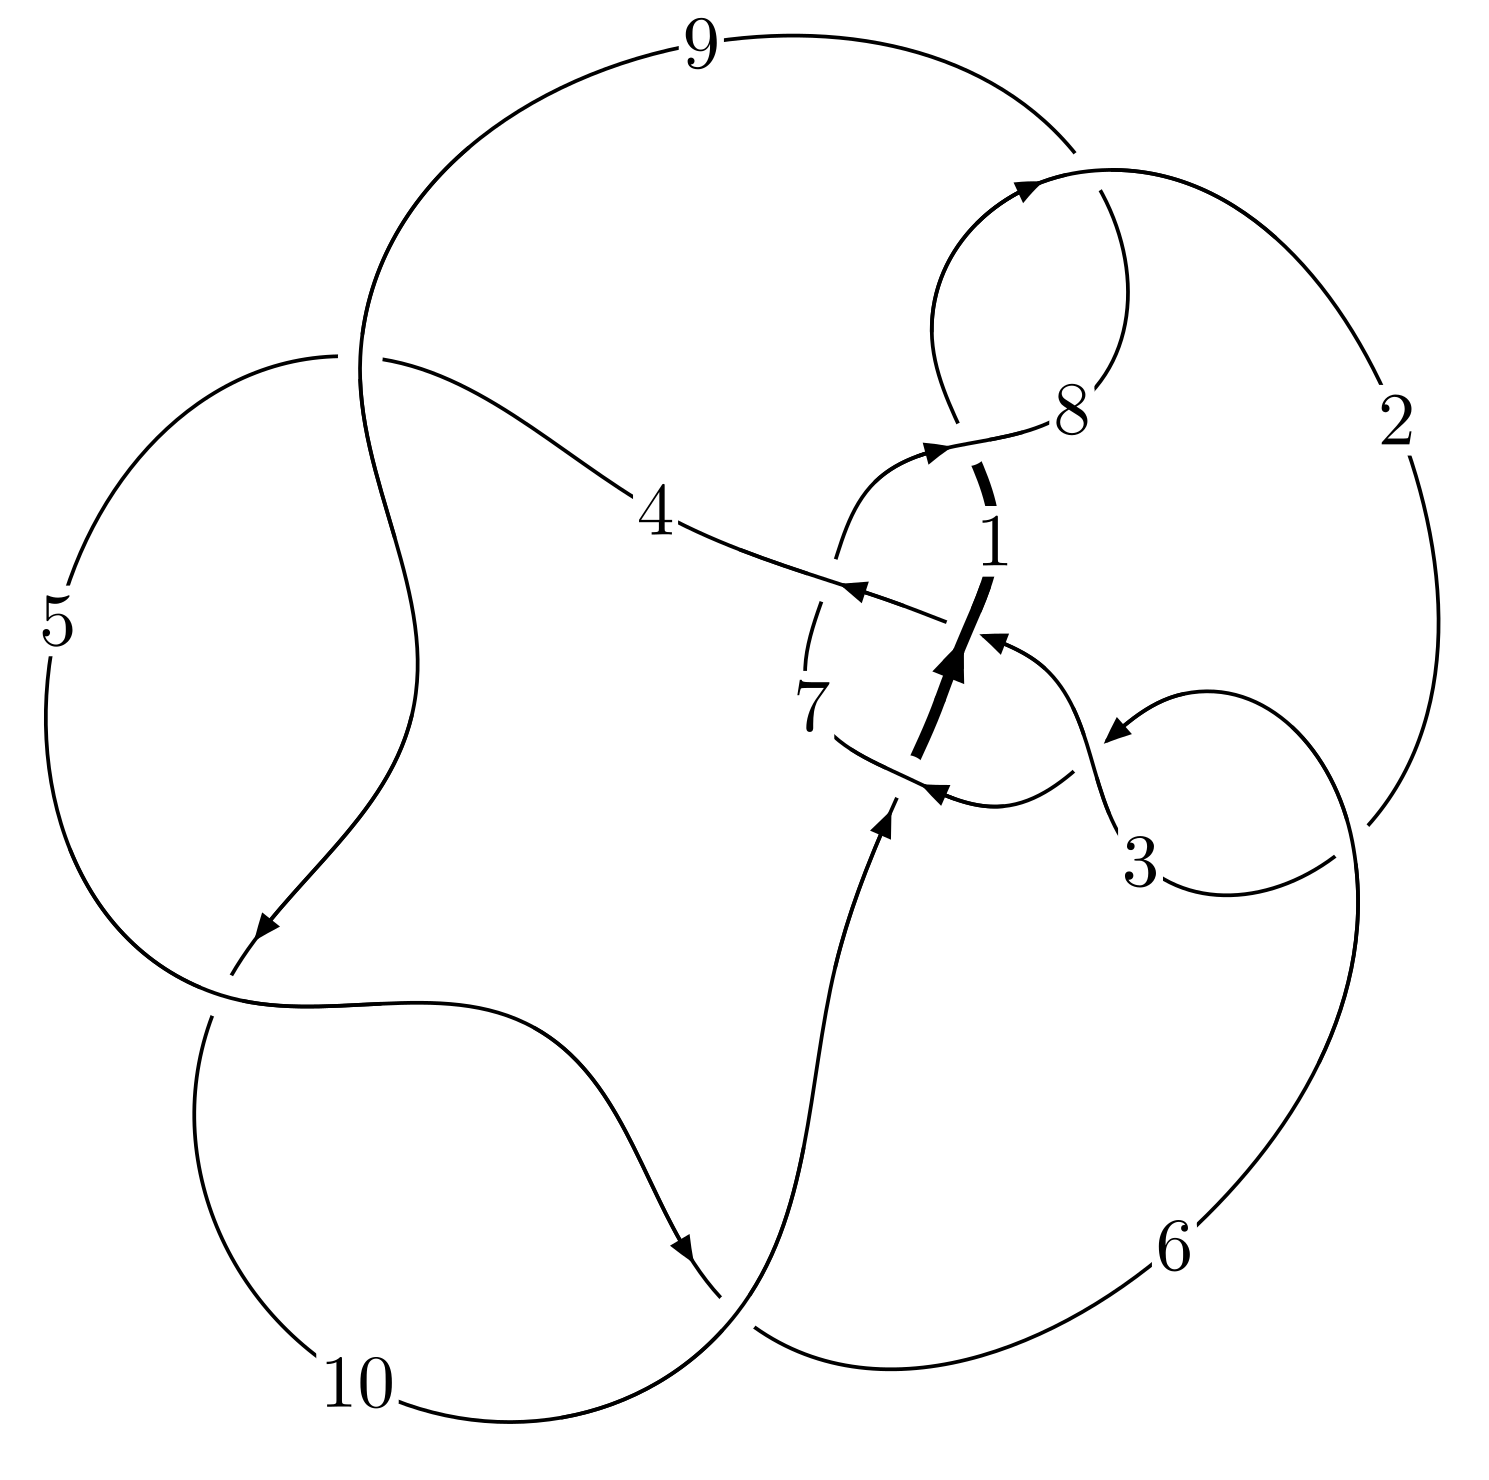
\includegraphics[width=112pt]{../../../GIT/diagram.site/Diagrams/png/188_10_104.png}\\
\ \ \ A knot diagram\footnotemark}&
\allowdisplaybreaks
\textbf{Linearized knot diagam} \\
\cline{2-2}
 &
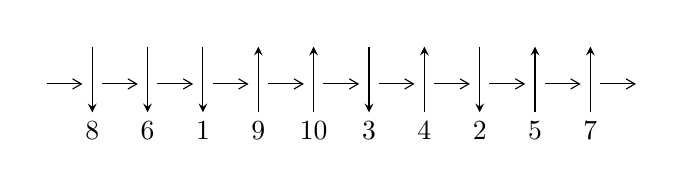
\begin{tikzpicture}[x=20pt, y=17pt]
	% nodes
	\node (C0) at (0, 0) {};
	\node (C1) at (1, 0) {};
	\node (C1U) at (1, +1) {};
	\node (C1D) at (1, -1) {8};

	\node (C2) at (2, 0) {};
	\node (C2U) at (2, +1) {};
	\node (C2D) at (2, -1) {6};

	\node (C3) at (3, 0) {};
	\node (C3U) at (3, +1) {};
	\node (C3D) at (3, -1) {1};

	\node (C4) at (4, 0) {};
	\node (C4U) at (4, +1) {};
	\node (C4D) at (4, -1) {9};

	\node (C5) at (5, 0) {};
	\node (C5U) at (5, +1) {};
	\node (C5D) at (5, -1) {10};

	\node (C6) at (6, 0) {};
	\node (C6U) at (6, +1) {};
	\node (C6D) at (6, -1) {3};

	\node (C7) at (7, 0) {};
	\node (C7U) at (7, +1) {};
	\node (C7D) at (7, -1) {4};

	\node (C8) at (8, 0) {};
	\node (C8U) at (8, +1) {};
	\node (C8D) at (8, -1) {2};

	\node (C9) at (9, 0) {};
	\node (C9U) at (9, +1) {};
	\node (C9D) at (9, -1) {5};

	\node (C10) at (10, 0) {};
	\node (C10U) at (10, +1) {};
	\node (C10D) at (10, -1) {7};
	\node (C11) at (11, 0) {};

	% arrows
	\draw[->,>={angle 60}]
	(C0) edge (C1) (C1) edge (C2) (C2) edge (C3) (C3) edge (C4) (C4) edge (C5) (C5) edge (C6) (C6) edge (C7) (C7) edge (C8) (C8) edge (C9) (C9) edge (C10) (C10) edge (C11) ;	\draw[->,>=stealth]
	(C1U) edge (C1D) (C2U) edge (C2D) (C3U) edge (C3D) (C4D) edge (C4U) (C5D) edge (C5U) (C6U) edge (C6D) (C7D) edge (C7U) (C8U) edge (C8D) (C9D) edge (C9U) (C10D) edge (C10U) ;
	\end{tikzpicture} \\
\hhline{~~} \\& 
\textbf{Solving Sequence} \\ \cline{2-2} 
 &
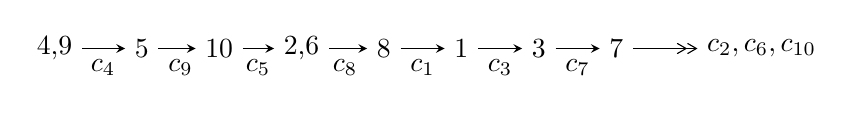
\begin{tikzpicture}[x=28pt, y=7pt]
	% node
	\node (A0) at (-1/8, 0) {4,9};
	\node (A1) at (1, 0) {5};
	\node (A2) at (2, 0) {10};
	\node (A3) at (49/16, 0) {2,6};
	\node (A4) at (33/8, 0) {8};
	\node (A5) at (41/8, 0) {1};
	\node (A6) at (49/8, 0) {3};
	\node (A7) at (57/8, 0) {7};
	\node (C1) at (1/2, -1) {$c_{4}$};
	\node (C2) at (3/2, -1) {$c_{9}$};
	\node (C3) at (5/2, -1) {$c_{5}$};
	\node (C4) at (29/8, -1) {$c_{8}$};
	\node (C5) at (37/8, -1) {$c_{1}$};
	\node (C6) at (45/8, -1) {$c_{3}$};
	\node (C7) at (53/8, -1) {$c_{7}$};
	\node (A8) at (9, 0) {$c_{2},c_{6},c_{10}$};

	% edge
	\draw[->,>=stealth]	
	(A0) edge (A1) (A1) edge (A2) (A2) edge (A3) (A3) edge (A4) (A4) edge (A5) (A5) edge (A6) (A6) edge (A7) ;
	\draw[->>,>={angle 60}]	
	(A7) edge (A8);
\end{tikzpicture} \\ 

\end{tabular} \\

\footnotetext{
The image of knot diagram is generated by the software ``\textbf{Draw programme}" developed by Andrew Bartholomew(\url{http://www.layer8.co.uk/maths/draw/index.htm\#Running-draw}), where we modified some parts for our purpose(\url{https://github.com/CATsTAILs/LinksPainter}).
}\phantom \\ \newline 
\centering \textbf{Ideals for irreducible components\footnotemark of $X_{\text{par}}$} 
 
\begin{align*}
I^u_{1}&=\langle 
- u^{14}-11 u^{13}+\cdots+4 b-20,\;41 u^{14}+221 u^{13}+\cdots+8 a+196,\\
\phantom{I^u_{1}}&\phantom{= \langle  }u^{15}+7 u^{14}+18 u^{13}+20 u^{12}+14 u^{11}+31 u^{10}+55 u^9+44 u^8+40 u^7+54 u^6+31 u^5+9 u^4+7 u^3-6 u^2+8\rangle \\
I^u_{2}&=\langle 
109 a^5 u^4+90 a^4 u^4+\cdots-83 a+145,\;-2 a^4 u^4-5 u^4 a^3+\cdots-18 a-1,\;u^5- u^4-2 u^3+u^2+u+1\rangle \\
I^u_{3}&=\langle 
- u^4+u^3+2 u^2+b- u,\;u^6+u^5-4 u^4-4 u^3+3 u^2+a+3 u+1,\;u^7-4 u^5- u^4+4 u^3+2 u^2-1\rangle \\
\\
\end{align*}
\raggedright * 3 irreducible components of $\dim_{\mathbb{C}}=0$, with total 52 representations.\\
\footnotetext{All coefficients of polynomials are rational numbers. But the coefficients are sometimes approximated in decimal forms when there is not enough margin.}
\newpage
\renewcommand{\arraystretch}{1}
\centering \section*{I. $I^u_{1}= \langle - u^{14}-11 u^{13}+\cdots+4 b-20,\;41 u^{14}+221 u^{13}+\cdots+8 a+196,\;u^{15}+7 u^{14}+\cdots-6 u^2+8 \rangle$}
\flushleft \textbf{(i) Arc colorings}\\
\begin{tabular}{m{7pt} m{180pt} m{7pt} m{180pt} }
\flushright $a_{4}=$&$\begin{pmatrix}1\\0\end{pmatrix}$ \\
\flushright $a_{9}=$&$\begin{pmatrix}0\\u\end{pmatrix}$ \\
\flushright $a_{5}=$&$\begin{pmatrix}1\\- u^2\end{pmatrix}$ \\
\flushright $a_{10}=$&$\begin{pmatrix}u\\- u^3+u\end{pmatrix}$ \\
\flushright $a_{2}=$&$\begin{pmatrix}-5.12500 u^{14}-27.6250 u^{13}+\cdots+15.5000 u-24.5000\\\frac{1}{4} u^{14}+\frac{11}{4} u^{13}+\cdots-\frac{9}{2} u+5\end{pmatrix}$ \\
\flushright $a_{6}=$&$\begin{pmatrix}- u^2+1\\u^4-2 u^2\end{pmatrix}$ \\
\flushright $a_{8}=$&$\begin{pmatrix}3 u^{14}+\frac{33}{2} u^{13}+\cdots-10 u+\frac{31}{2}\\\frac{3}{2} u^{14}+7 u^{13}+\cdots+\frac{1}{2} u+4\end{pmatrix}$ \\
\flushright $a_{1}=$&$\begin{pmatrix}-8 u^{14}-\frac{179}{4} u^{13}+\cdots+\frac{125}{4} u-44\\\frac{17}{4} u^{14}+\frac{97}{4} u^{13}+\cdots-19 u+26\end{pmatrix}$ \\
\flushright $a_{3}=$&$\begin{pmatrix}\frac{53}{8} u^{14}+\frac{301}{8} u^{13}+\cdots-26 u+\frac{77}{2}\\-\frac{15}{4} u^{14}-\frac{89}{4} u^{13}+\cdots+\frac{47}{2} u-27\end{pmatrix}$ \\
\flushright $a_{7}=$&$\begin{pmatrix}\frac{3}{2} u^{14}+\frac{19}{2} u^{13}+\cdots-\frac{21}{2} u+\frac{23}{2}\\\frac{3}{2} u^{14}+7 u^{13}+\cdots+\frac{1}{2} u+4\end{pmatrix}$\\&\end{tabular}
\flushleft \textbf{(ii) Obstruction class $= -1$}\\~\\
\flushleft \textbf{(iii) Cusp Shapes $= 10 u^{14}+59 u^{13}+113 u^{12}+66 u^{11}+54 u^{10}+245 u^9+267 u^8+113 u^7+251 u^6+241 u^5+11 u^4+66 u^3-7 u^2-60 u+74$}\\~\\
\newpage\renewcommand{\arraystretch}{1}
\flushleft \textbf{(iv) u-Polynomials at the component}\newline \\
\begin{tabular}{m{50pt}|m{274pt}}
Crossings & \hspace{64pt}u-Polynomials at each crossing \\
\hline $$\begin{aligned}c_{1},c_{2},c_{6}\\c_{8}\end{aligned}$$&$\begin{aligned}
&u^{15}+u^{14}+\cdots-3 u^3-1
\end{aligned}$\\
\hline $$\begin{aligned}c_{3}\end{aligned}$$&$\begin{aligned}
&u^{15}-12 u^{14}+\cdots+240 u-32
\end{aligned}$\\
\hline $$\begin{aligned}c_{4},c_{5},c_{9}\end{aligned}$$&$\begin{aligned}
&u^{15}+7 u^{14}+\cdots-6 u^2+8
\end{aligned}$\\
\hline $$\begin{aligned}c_{7},c_{10}\end{aligned}$$&$\begin{aligned}
&u^{15}-3 u^{13}+\cdots+u+1
\end{aligned}$\\
\hline
\end{tabular}\\~\\
\newpage\renewcommand{\arraystretch}{1}
\flushleft \textbf{(v) Riley Polynomials at the component}\newline \\
\begin{tabular}{m{50pt}|m{274pt}}
Crossings & \hspace{64pt}Riley Polynomials at each crossing \\
\hline $$\begin{aligned}c_{1},c_{2},c_{6}\\c_{8}\end{aligned}$$&$\begin{aligned}
&y^{15}-9 y^{14}+\cdots+4 y^2-1
\end{aligned}$\\
\hline $$\begin{aligned}c_{3}\end{aligned}$$&$\begin{aligned}
&y^{15}-4 y^{14}+\cdots-1280 y-1024
\end{aligned}$\\
\hline $$\begin{aligned}c_{4},c_{5},c_{9}\end{aligned}$$&$\begin{aligned}
&y^{15}-13 y^{14}+\cdots+96 y-64
\end{aligned}$\\
\hline $$\begin{aligned}c_{7},c_{10}\end{aligned}$$&$\begin{aligned}
&y^{15}-6 y^{14}+\cdots+13 y-1
\end{aligned}$\\
\hline
\end{tabular}\\~\\
\newpage\flushleft \textbf{(vi) Complex Volumes and Cusp Shapes}
$$\begin{array}{c|c|c}  
\text{Solutions to }I^u_{1}& \I (\text{vol} + \sqrt{-1}CS) & \text{Cusp shape}\\
 \hline 
\begin{aligned}
u &= \phantom{-}0.388466 + 0.947688 I \\
a &= \phantom{-}0.050943 - 1.350340 I \\
b &= -0.47742 - 1.71628 I\end{aligned}
 & -5.82203 + 9.38410 I & -3.97952 - 7.17475 I \\ \hline\begin{aligned}
u &= \phantom{-}0.388466 - 0.947688 I \\
a &= \phantom{-}0.050943 + 1.350340 I \\
b &= -0.47742 + 1.71628 I\end{aligned}
 & -5.82203 - 9.38410 I & -3.97952 + 7.17475 I \\ \hline\begin{aligned}
u &= -0.101121 + 0.829275 I \\
a &= \phantom{-}0.467120 + 0.846136 I \\
b &= -0.108197 + 1.248190 I\end{aligned}
 & -1.32635 + 1.58430 I & \phantom{-}2.05695 - 3.17357 I \\ \hline\begin{aligned}
u &= -0.101121 - 0.829275 I \\
a &= \phantom{-}0.467120 - 0.846136 I \\
b &= -0.108197 - 1.248190 I\end{aligned}
 & -1.32635 - 1.58430 I & \phantom{-}2.05695 + 3.17357 I \\ \hline\begin{aligned}
u &= \phantom{-}0.922792 + 0.829091 I \\
a &= -0.839212 + 0.446521 I \\
b &= \phantom{-}0.265387 + 1.302840 I\end{aligned}
 & -4.34026 - 3.41455 I & -3.26031 + 4.30453 I \\ \hline\begin{aligned}
u &= \phantom{-}0.922792 - 0.829091 I \\
a &= -0.839212 - 0.446521 I \\
b &= \phantom{-}0.265387 - 1.302840 I\end{aligned}
 & -4.34026 + 3.41455 I & -3.26031 - 4.30453 I \\ \hline\begin{aligned}
u &= \phantom{-}0.528410 + 0.302526 I \\
a &= \phantom{-}0.715576 + 0.595124 I \\
b &= \phantom{-}0.246839 - 0.030877 I\end{aligned}
 & \phantom{-}1.036950 + 0.848562 I & \phantom{-}5.31510 - 2.72513 I \\ \hline\begin{aligned}
u &= \phantom{-}0.528410 - 0.302526 I \\
a &= \phantom{-}0.715576 - 0.595124 I \\
b &= \phantom{-}0.246839 + 0.030877 I\end{aligned}
 & \phantom{-}1.036950 - 0.848562 I & \phantom{-}5.31510 + 2.72513 I \\ \hline\begin{aligned}
u &= -1.38123 + 0.42191 I \\
a &= -0.521626 - 0.558152 I \\
b &= \phantom{-}1.14450 - 1.53934 I\end{aligned}
 & \phantom{-}2.89422 - 6.37595 I & \phantom{-}2.35312 + 7.90831 I \\ \hline\begin{aligned}
u &= -1.38123 - 0.42191 I \\
a &= -0.521626 + 0.558152 I \\
b &= \phantom{-}1.14450 + 1.53934 I\end{aligned}
 & \phantom{-}2.89422 + 6.37595 I & \phantom{-}2.35312 - 7.90831 I\\
 \hline 
 \end{array}$$\newpage$$\begin{array}{c|c|c}  
\text{Solutions to }I^u_{1}& \I (\text{vol} + \sqrt{-1}CS) & \text{Cusp shape}\\
 \hline 
\begin{aligned}
u &= -1.48635 + 0.07152 I \\
a &= \phantom{-}0.098561 - 0.589973 I \\
b &= \phantom{-}0.379744 - 0.426871 I\end{aligned}
 & \phantom{-}7.67422 - 2.17377 I & \phantom{-}7.19312 + 2.21789 I \\ \hline\begin{aligned}
u &= -1.48635 - 0.07152 I \\
a &= \phantom{-}0.098561 + 0.589973 I \\
b &= \phantom{-}0.379744 + 0.426871 I\end{aligned}
 & \phantom{-}7.67422 + 2.17377 I & \phantom{-}7.19312 - 2.21789 I \\ \hline\begin{aligned}
u &= -1.49023 + 0.36505 I \\
a &= \phantom{-}0.758806 + 0.630997 I \\
b &= -1.13261 + 1.70886 I\end{aligned}
 & \phantom{-}0.18522 - 14.10710 I & -0.21037 + 7.77333 I \\ \hline\begin{aligned}
u &= -1.49023 - 0.36505 I \\
a &= \phantom{-}0.758806 - 0.630997 I \\
b &= -1.13261 - 1.70886 I\end{aligned}
 & \phantom{-}0.18522 + 14.10710 I & -0.21037 - 7.77333 I \\ \hline\begin{aligned}
u &= -1.76149\phantom{ +0.000000I} \\
a &= -0.460333\phantom{ +0.000000I} \\
b &= \phantom{-}0.363500\phantom{ +0.000000I}\end{aligned}
 & \phantom{-}5.97579\phantom{ +0.000000I} & -5.93620\phantom{ +0.000000I}\\
 \hline 
 \end{array}$$\newpage\newpage\renewcommand{\arraystretch}{1}
\centering \section*{II. $I^u_{2}= \langle 109 a^5 u^4+90 a^4 u^4+\cdots-83 a+145,\;-2 a^4 u^4-5 u^4 a^3+\cdots-18 a-1,\;u^5- u^4-2 u^3+u^2+u+1 \rangle$}
\flushleft \textbf{(i) Arc colorings}\\
\begin{tabular}{m{7pt} m{180pt} m{7pt} m{180pt} }
\flushright $a_{4}=$&$\begin{pmatrix}1\\0\end{pmatrix}$ \\
\flushright $a_{9}=$&$\begin{pmatrix}0\\u\end{pmatrix}$ \\
\flushright $a_{5}=$&$\begin{pmatrix}1\\- u^2\end{pmatrix}$ \\
\flushright $a_{10}=$&$\begin{pmatrix}u\\- u^3+u\end{pmatrix}$ \\
\flushright $a_{2}=$&$\begin{pmatrix}a\\-0.947826 a^{5} u^{4}-0.782609 a^{4} u^{4}+\cdots+0.721739 a-1.26087\end{pmatrix}$ \\
\flushright $a_{6}=$&$\begin{pmatrix}- u^2+1\\u^4-2 u^2\end{pmatrix}$ \\
\flushright $a_{8}=$&$\begin{pmatrix}a^2 u\\1.56522 a^{5} u^{4}-0.278261 a^{4} u^{4}+\cdots-0.547826 a+0.973913\end{pmatrix}$ \\
\flushright $a_{1}=$&$\begin{pmatrix}- a^3 u^2+a\\-0.504348 a^{5} u^{4}-1.63478 a^{4} u^{4}+\cdots+0.556522 a-0.278261\end{pmatrix}$ \\
\flushright $a_{3}=$&$\begin{pmatrix}1.39130 a^{5} u^{4}+0.330435 a^{4} u^{4}+\cdots+1.71304 a+0.843478\\-1.23478 a^{5} u^{4}-0.678261 a^{4} u^{4}+\cdots+0.452174 a+0.373913\end{pmatrix}$ \\
\flushright $a_{7}=$&$\begin{pmatrix}-1.56522 a^{5} u^{4}+0.278261 a^{4} u^{4}+\cdots+0.547826 a-0.973913\\1.56522 a^{5} u^{4}-0.278261 a^{4} u^{4}+\cdots-0.547826 a+0.973913\end{pmatrix}$\\&\end{tabular}
\flushleft \textbf{(ii) Obstruction class $= -1$}\\~\\
\flushleft \textbf{(iii) Cusp Shapes $= \frac{232}{115} a^5 u^4+\frac{752}{115} a^4 u^4+\cdots-\frac{256}{115} a-\frac{102}{115}$}\\~\\
\newpage\renewcommand{\arraystretch}{1}
\flushleft \textbf{(iv) u-Polynomials at the component}\newline \\
\begin{tabular}{m{50pt}|m{274pt}}
Crossings & \hspace{64pt}u-Polynomials at each crossing \\
\hline $$\begin{aligned}c_{1},c_{2},c_{6}\\c_{8}\end{aligned}$$&$\begin{aligned}
&u^{30}- u^{29}+\cdots-64 u-7
\end{aligned}$\\
\hline $$\begin{aligned}c_{3}\end{aligned}$$&$\begin{aligned}
&(u^3+u^2-1)^{10}
\end{aligned}$\\
\hline $$\begin{aligned}c_{4},c_{5},c_{9}\end{aligned}$$&$\begin{aligned}
&(u^5- u^4-2 u^3+u^2+u+1)^6
\end{aligned}$\\
\hline $$\begin{aligned}c_{7},c_{10}\end{aligned}$$&$\begin{aligned}
&u^{30}-3 u^{29}+\cdots-14 u-1
\end{aligned}$\\
\hline
\end{tabular}\\~\\
\newpage\renewcommand{\arraystretch}{1}
\flushleft \textbf{(v) Riley Polynomials at the component}\newline \\
\begin{tabular}{m{50pt}|m{274pt}}
Crossings & \hspace{64pt}Riley Polynomials at each crossing \\
\hline $$\begin{aligned}c_{1},c_{2},c_{6}\\c_{8}\end{aligned}$$&$\begin{aligned}
&y^{30}-21 y^{29}+\cdots-1884 y+49
\end{aligned}$\\
\hline $$\begin{aligned}c_{3}\end{aligned}$$&$\begin{aligned}
&(y^3- y^2+2 y-1)^{10}
\end{aligned}$\\
\hline $$\begin{aligned}c_{4},c_{5},c_{9}\end{aligned}$$&$\begin{aligned}
&(y^5-5 y^4+8 y^3-3 y^2- y-1)^6
\end{aligned}$\\
\hline $$\begin{aligned}c_{7},c_{10}\end{aligned}$$&$\begin{aligned}
&y^{30}+7 y^{29}+\cdots-116 y+1
\end{aligned}$\\
\hline
\end{tabular}\\~\\
\newpage\flushleft \textbf{(vi) Complex Volumes and Cusp Shapes}
$$\begin{array}{c|c|c}  
\text{Solutions to }I^u_{2}& \I (\text{vol} + \sqrt{-1}CS) & \text{Cusp shape}\\
 \hline 
\begin{aligned}
u &= -1.21774\phantom{ +0.000000I} \\
a &= -0.806664 + 0.705849 I \\
b &= \phantom{-}0.41170 + 1.41665 I\end{aligned}
 & \phantom{-}0.49041 + 2.82812 I & -1.00910 - 2.97945 I \\ \hline\begin{aligned}
u &= -1.21774\phantom{ +0.000000I} \\
a &= -0.806664 - 0.705849 I \\
b &= \phantom{-}0.41170 - 1.41665 I\end{aligned}
 & \phantom{-}0.49041 - 2.82812 I & -1.00910 + 2.97945 I \\ \hline\begin{aligned}
u &= -1.21774\phantom{ +0.000000I} \\
a &= \phantom{-}1.23353\phantom{ +0.000000I} \\
b &= -2.05678\phantom{ +0.000000I}\end{aligned}
 & -3.64718\phantom{ +0.000000I} & -7.53840\phantom{ +0.000000I} \\ \hline\begin{aligned}
u &= -1.21774\phantom{ +0.000000I} \\
a &= \phantom{-}0.671225 + 0.117277 I \\
b &= -0.96834 + 1.96626 I\end{aligned}
 & \phantom{-}0.49041 + 2.82812 I & -1.00910 - 2.97945 I \\ \hline\begin{aligned}
u &= -1.21774\phantom{ +0.000000I} \\
a &= \phantom{-}0.671225 - 0.117277 I \\
b &= -0.96834 - 1.96626 I\end{aligned}
 & \phantom{-}0.49041 - 2.82812 I & -1.00910 + 2.97945 I \\ \hline\begin{aligned}
u &= -1.21774\phantom{ +0.000000I} \\
a &= -1.59237\phantom{ +0.000000I} \\
b &= \phantom{-}0.582023\phantom{ +0.000000I}\end{aligned}
 & -3.64718\phantom{ +0.000000I} & -7.53840\phantom{ +0.000000I} \\ \hline\begin{aligned}
u &= -0.309916 + 0.549911 I \\
a &= -1.25942 + 0.90741 I \\
b &= -0.129260 - 0.273797 I\end{aligned}
 & -1.58157 - 4.35870 I & -1.97513 + 7.41010 I \\ \hline\begin{aligned}
u &= -0.309916 + 0.549911 I \\
a &= \phantom{-}1.21172 + 1.02695 I \\
b &= -0.218320 + 1.108690 I\end{aligned}
 & -1.58157 + 1.29754 I & -1.97513 + 1.45120 I \\ \hline\begin{aligned}
u &= -0.309916 + 0.549911 I \\
a &= \phantom{-}0.048773 + 0.350100 I \\
b &= -0.820174 + 0.651930 I\end{aligned}
 & -1.58157 + 1.29754 I & -1.97513 + 1.45120 I \\ \hline\begin{aligned}
u &= -0.309916 + 0.549911 I \\
a &= -0.37583 - 1.80799 I \\
b &= \phantom{-}0.54889 - 1.72674 I\end{aligned}
 & -1.58157 - 4.35870 I & -1.97513 + 7.41010 I\\
 \hline 
 \end{array}$$\newpage$$\begin{array}{c|c|c}  
\text{Solutions to }I^u_{2}& \I (\text{vol} + \sqrt{-1}CS) & \text{Cusp shape}\\
 \hline 
\begin{aligned}
u &= -0.309916 + 0.549911 I \\
a &= -0.96996 - 1.69646 I \\
b &= -0.67455 - 1.32965 I\end{aligned}
 & -5.71916 - 1.53058 I & -8.50440 + 4.43065 I \\ \hline\begin{aligned}
u &= -0.309916 + 0.549911 I \\
a &= \phantom{-}0.47350 + 2.32765 I \\
b &= -0.145272 + 1.011820 I\end{aligned}
 & -5.71916 - 1.53058 I & -8.50440 + 4.43065 I \\ \hline\begin{aligned}
u &= -0.309916 - 0.549911 I \\
a &= -1.25942 - 0.90741 I \\
b &= -0.129260 + 0.273797 I\end{aligned}
 & -1.58157 + 4.35870 I & -1.97513 - 7.41010 I \\ \hline\begin{aligned}
u &= -0.309916 - 0.549911 I \\
a &= \phantom{-}1.21172 - 1.02695 I \\
b &= -0.218320 - 1.108690 I\end{aligned}
 & -1.58157 - 1.29754 I & -1.97513 - 1.45120 I \\ \hline\begin{aligned}
u &= -0.309916 - 0.549911 I \\
a &= \phantom{-}0.048773 - 0.350100 I \\
b &= -0.820174 - 0.651930 I\end{aligned}
 & -1.58157 - 1.29754 I & -1.97513 - 1.45120 I \\ \hline\begin{aligned}
u &= -0.309916 - 0.549911 I \\
a &= -0.37583 + 1.80799 I \\
b &= \phantom{-}0.54889 + 1.72674 I\end{aligned}
 & -1.58157 + 4.35870 I & -1.97513 - 7.41010 I \\ \hline\begin{aligned}
u &= -0.309916 - 0.549911 I \\
a &= -0.96996 + 1.69646 I \\
b &= -0.67455 + 1.32965 I\end{aligned}
 & -5.71916 + 1.53058 I & -8.50440 - 4.43065 I \\ \hline\begin{aligned}
u &= -0.309916 - 0.549911 I \\
a &= \phantom{-}0.47350 - 2.32765 I \\
b &= -0.145272 - 1.011820 I\end{aligned}
 & -5.71916 + 1.53058 I & -8.50440 - 4.43065 I \\ \hline\begin{aligned}
u &= \phantom{-}1.41878 + 0.21917 I \\
a &= -0.837994 + 0.477676 I \\
b &= \phantom{-}1.48326 + 1.70876 I\end{aligned}
 & \phantom{-}3.96189 + 7.22895 I & \phantom{-}2.25407 - 6.47803 I \\ \hline\begin{aligned}
u &= \phantom{-}1.41878 + 0.21917 I \\
a &= -0.265271 - 0.909026 I \\
b &= -0.218527 - 0.470543 I\end{aligned}
 & \phantom{-}3.96189 + 7.22895 I & \phantom{-}2.25407 - 6.47803 I\\
 \hline 
 \end{array}$$\newpage$$\begin{array}{c|c|c}  
\text{Solutions to }I^u_{2}& \I (\text{vol} + \sqrt{-1}CS) & \text{Cusp shape}\\
 \hline 
\begin{aligned}
u &= \phantom{-}1.41878 + 0.21917 I \\
a &= \phantom{-}0.772271 - 0.730462 I \\
b &= -0.335807 - 1.278970 I\end{aligned}
 & -0.17569 + 4.40083 I & -4.27520 - 3.49859 I \\ \hline\begin{aligned}
u &= \phantom{-}1.41878 + 0.21917 I \\
a &= \phantom{-}0.696565 - 0.364337 I \\
b &= -1.33013 - 0.90847 I\end{aligned}
 & \phantom{-}3.96189 + 1.57271 I & \phantom{-}2.25407 - 0.51914 I \\ \hline\begin{aligned}
u &= \phantom{-}1.41878 + 0.21917 I \\
a &= -0.666236 + 0.232053 I \\
b &= -0.10143 + 1.90226 I\end{aligned}
 & -0.17569 + 4.40083 I & -4.27520 - 3.49859 I \\ \hline\begin{aligned}
u &= \phantom{-}1.41878 + 0.21917 I \\
a &= \phantom{-}0.486743 + 0.419449 I \\
b &= -0.264664 + 0.140760 I\end{aligned}
 & \phantom{-}3.96189 + 1.57271 I & \phantom{-}2.25407 - 0.51914 I \\ \hline\begin{aligned}
u &= \phantom{-}1.41878 - 0.21917 I \\
a &= -0.837994 - 0.477676 I \\
b &= \phantom{-}1.48326 - 1.70876 I\end{aligned}
 & \phantom{-}3.96189 - 7.22895 I & \phantom{-}2.25407 + 6.47803 I \\ \hline\begin{aligned}
u &= \phantom{-}1.41878 - 0.21917 I \\
a &= -0.265271 + 0.909026 I \\
b &= -0.218527 + 0.470543 I\end{aligned}
 & \phantom{-}3.96189 - 7.22895 I & \phantom{-}2.25407 + 6.47803 I \\ \hline\begin{aligned}
u &= \phantom{-}1.41878 - 0.21917 I \\
a &= \phantom{-}0.772271 + 0.730462 I \\
b &= -0.335807 + 1.278970 I\end{aligned}
 & -0.17569 - 4.40083 I & -4.27520 + 3.49859 I \\ \hline\begin{aligned}
u &= \phantom{-}1.41878 - 0.21917 I \\
a &= \phantom{-}0.696565 + 0.364337 I \\
b &= -1.33013 + 0.90847 I\end{aligned}
 & \phantom{-}3.96189 - 1.57271 I & \phantom{-}2.25407 + 0.51914 I \\ \hline\begin{aligned}
u &= \phantom{-}1.41878 - 0.21917 I \\
a &= -0.666236 - 0.232053 I \\
b &= -0.10143 - 1.90226 I\end{aligned}
 & -0.17569 - 4.40083 I & -4.27520 + 3.49859 I \\ \hline\begin{aligned}
u &= \phantom{-}1.41878 - 0.21917 I \\
a &= \phantom{-}0.486743 - 0.419449 I \\
b &= -0.264664 - 0.140760 I\end{aligned}
 & \phantom{-}3.96189 - 1.57271 I & \phantom{-}2.25407 + 0.51914 I\\
 \hline 
 \end{array}$$\newpage\newpage\renewcommand{\arraystretch}{1}
\centering \section*{III. $I^u_{3}= \langle - u^4+u^3+2 u^2+b- u,\;u^6+u^5-4 u^4-4 u^3+3 u^2+a+3 u+1,\;u^7-4 u^5- u^4+4 u^3+2 u^2-1 \rangle$}
\flushleft \textbf{(i) Arc colorings}\\
\begin{tabular}{m{7pt} m{180pt} m{7pt} m{180pt} }
\flushright $a_{4}=$&$\begin{pmatrix}1\\0\end{pmatrix}$ \\
\flushright $a_{9}=$&$\begin{pmatrix}0\\u\end{pmatrix}$ \\
\flushright $a_{5}=$&$\begin{pmatrix}1\\- u^2\end{pmatrix}$ \\
\flushright $a_{10}=$&$\begin{pmatrix}u\\- u^3+u\end{pmatrix}$ \\
\flushright $a_{2}=$&$\begin{pmatrix}- u^6- u^5+4 u^4+4 u^3-3 u^2-3 u-1\\u^4- u^3-2 u^2+u\end{pmatrix}$ \\
\flushright $a_{6}=$&$\begin{pmatrix}- u^2+1\\u^4-2 u^2\end{pmatrix}$ \\
\flushright $a_{8}=$&$\begin{pmatrix}u^6-4 u^4-2 u^3+4 u^2+4 u+1\\u^6-3 u^4- u^3+2 u^2+u\end{pmatrix}$ \\
\flushright $a_{1}=$&$\begin{pmatrix}u^6+u^5-3 u^4-4 u^3+3 u+2\\- u^3+2 u\end{pmatrix}$ \\
\flushright $a_{3}=$&$\begin{pmatrix}- u^6- u^5+4 u^4+4 u^3-3 u^2-3 u\\- u^6+4 u^4-4 u^2\end{pmatrix}$ \\
\flushright $a_{7}=$&$\begin{pmatrix}- u^4- u^3+2 u^2+3 u+1\\u^6-3 u^4- u^3+2 u^2+u\end{pmatrix}$\\&\end{tabular}
\flushleft \textbf{(ii) Obstruction class $= 1$}\\~\\
\flushleft \textbf{(iii) Cusp Shapes $= -2 u^6+u^5+3 u^4+3 u^3+7 u^2-5 u-8$}\\~\\
\newpage\renewcommand{\arraystretch}{1}
\flushleft \textbf{(iv) u-Polynomials at the component}\newline \\
\begin{tabular}{m{50pt}|m{274pt}}
Crossings & \hspace{64pt}u-Polynomials at each crossing \\
\hline $$\begin{aligned}c_{1},c_{6}\end{aligned}$$&$\begin{aligned}
&u^7- u^6-3 u^5+3 u^4+2 u^3-3 u^2- u+1
\end{aligned}$\\
\hline $$\begin{aligned}c_{2},c_{8}\end{aligned}$$&$\begin{aligned}
&u^7+u^6-3 u^5-3 u^4+2 u^3+3 u^2- u-1
\end{aligned}$\\
\hline $$\begin{aligned}c_{3}\end{aligned}$$&$\begin{aligned}
&u^7+3 u^6+3 u^5- u^4-4 u^3-2 u^2+1
\end{aligned}$\\
\hline $$\begin{aligned}c_{4},c_{5}\end{aligned}$$&$\begin{aligned}
&u^7-4 u^5- u^4+4 u^3+2 u^2-1
\end{aligned}$\\
\hline $$\begin{aligned}c_{7},c_{10}\end{aligned}$$&$\begin{aligned}
&u^7+u^4-2 u^3-1
\end{aligned}$\\
\hline $$\begin{aligned}c_{9}\end{aligned}$$&$\begin{aligned}
&u^7-4 u^5+u^4+4 u^3-2 u^2+1
\end{aligned}$\\
\hline
\end{tabular}\\~\\
\newpage\renewcommand{\arraystretch}{1}
\flushleft \textbf{(v) Riley Polynomials at the component}\newline \\
\begin{tabular}{m{50pt}|m{274pt}}
Crossings & \hspace{64pt}Riley Polynomials at each crossing \\
\hline $$\begin{aligned}c_{1},c_{2},c_{6}\\c_{8}\end{aligned}$$&$\begin{aligned}
&y^7-7 y^6+19 y^5-29 y^4+30 y^3-19 y^2+7 y-1
\end{aligned}$\\
\hline $$\begin{aligned}c_{3}\end{aligned}$$&$\begin{aligned}
&y^7-3 y^6+7 y^5-13 y^4+6 y^3-2 y^2+4 y-1
\end{aligned}$\\
\hline $$\begin{aligned}c_{4},c_{5},c_{9}\end{aligned}$$&$\begin{aligned}
&y^7-8 y^6+24 y^5-33 y^4+20 y^3-6 y^2+4 y-1
\end{aligned}$\\
\hline $$\begin{aligned}c_{7},c_{10}\end{aligned}$$&$\begin{aligned}
&y^7-4 y^5- y^4+4 y^3+2 y^2-1
\end{aligned}$\\
\hline
\end{tabular}\\~\\
\newpage\flushleft \textbf{(vi) Complex Volumes and Cusp Shapes}
$$\begin{array}{c|c|c}  
\text{Solutions to }I^u_{3}& \I (\text{vol} + \sqrt{-1}CS) & \text{Cusp shape}\\
 \hline 
\begin{aligned}
u &= \phantom{-}1.25920\phantom{ +0.000000I} \\
a &= \phantom{-}1.35619\phantom{ +0.000000I} \\
b &= -1.39446\phantom{ +0.000000I}\end{aligned}
 & -2.88904\phantom{ +0.000000I} & \phantom{-}5.52810\phantom{ +0.000000I} \\ \hline\begin{aligned}
u &= -0.401963 + 0.546430 I \\
a &= \phantom{-}1.019580 + 0.650467 I \\
b &= -0.59726 + 1.44367 I\end{aligned}
 & -2.11479 + 2.13385 I & -6.73578 - 5.40456 I \\ \hline\begin{aligned}
u &= -0.401963 - 0.546430 I \\
a &= \phantom{-}1.019580 - 0.650467 I \\
b &= -0.59726 - 1.44367 I\end{aligned}
 & -2.11479 - 2.13385 I & -6.73578 + 5.40456 I \\ \hline\begin{aligned}
u &= -1.346460 + 0.204423 I \\
a &= -0.556014 - 0.539828 I \\
b &= \phantom{-}0.21748 - 1.74792 I\end{aligned}
 & \phantom{-}1.45010 - 4.82255 I & \phantom{-}1.50641 + 5.81707 I \\ \hline\begin{aligned}
u &= -1.346460 - 0.204423 I \\
a &= -0.556014 + 0.539828 I \\
b &= \phantom{-}0.21748 + 1.74792 I\end{aligned}
 & \phantom{-}1.45010 + 4.82255 I & \phantom{-}1.50641 - 5.81707 I \\ \hline\begin{aligned}
u &= \phantom{-}0.552010\phantom{ +0.000000I} \\
a &= -2.60549\phantom{ +0.000000I} \\
b &= -0.132774\phantom{ +0.000000I}\end{aligned}
 & -5.57629\phantom{ +0.000000I} & -7.84920\phantom{ +0.000000I} \\ \hline\begin{aligned}
u &= \phantom{-}1.68564\phantom{ +0.000000I} \\
a &= \phantom{-}0.322173\phantom{ +0.000000I} \\
b &= -0.713207\phantom{ +0.000000I}\end{aligned}
 & \phantom{-}6.50483\phantom{ +0.000000I} & \phantom{-}9.77980\phantom{ +0.000000I}\\
 \hline 
 \end{array}$$\newpage
\newpage\renewcommand{\arraystretch}{1}
\centering \section*{ IV. u-Polynomials}
\begin{tabular}{m{50pt}|m{274pt}}
Crossings & \hspace{64pt}u-Polynomials at each crossing \\
\hline $$\begin{aligned}c_{1},c_{6}\end{aligned}$$&$\begin{aligned}
&(u^7- u^6+\cdots- u+1)(u^{15}+u^{14}+\cdots-3 u^3-1)\\
&\cdot(u^{30}- u^{29}+\cdots-64 u-7)
\end{aligned}$\\
\hline $$\begin{aligned}c_{2},c_{8}\end{aligned}$$&$\begin{aligned}
&(u^7+u^6+\cdots- u-1)(u^{15}+u^{14}+\cdots-3 u^3-1)\\
&\cdot(u^{30}- u^{29}+\cdots-64 u-7)
\end{aligned}$\\
\hline $$\begin{aligned}c_{3}\end{aligned}$$&$\begin{aligned}
&(u^3+u^2-1)^{10}(u^7+3 u^6+3 u^5- u^4-4 u^3-2 u^2+1)\\
&\cdot(u^{15}-12 u^{14}+\cdots+240 u-32)
\end{aligned}$\\
\hline $$\begin{aligned}c_{4},c_{5}\end{aligned}$$&$\begin{aligned}
&(u^5- u^4-2 u^3+u^2+u+1)^6(u^7-4 u^5- u^4+4 u^3+2 u^2-1)\\
&\cdot(u^{15}+7 u^{14}+\cdots-6 u^2+8)
\end{aligned}$\\
\hline $$\begin{aligned}c_{7},c_{10}\end{aligned}$$&$\begin{aligned}
&(u^7+u^4-2 u^3-1)(u^{15}-3 u^{13}+\cdots+u+1)(u^{30}-3 u^{29}+\cdots-14 u-1)
\end{aligned}$\\
\hline $$\begin{aligned}c_{9}\end{aligned}$$&$\begin{aligned}
&(u^5- u^4-2 u^3+u^2+u+1)^6(u^7-4 u^5+u^4+4 u^3-2 u^2+1)\\
&\cdot(u^{15}+7 u^{14}+\cdots-6 u^2+8)
\end{aligned}$\\
\hline
\end{tabular}\newpage\renewcommand{\arraystretch}{1}
\centering \section*{ V. Riley Polynomials}
\begin{tabular}{m{50pt}|m{274pt}}
Crossings & \hspace{64pt}Riley Polynomials at each crossing \\
\hline $$\begin{aligned}c_{1},c_{2},c_{6}\\c_{8}\end{aligned}$$&$\begin{aligned}
&(y^7-7 y^6+19 y^5-29 y^4+30 y^3-19 y^2+7 y-1)\\
&\cdot(y^{15}-9 y^{14}+\cdots+4 y^2-1)(y^{30}-21 y^{29}+\cdots-1884 y+49)
\end{aligned}$\\
\hline $$\begin{aligned}c_{3}\end{aligned}$$&$\begin{aligned}
&(y^3- y^2+2 y-1)^{10}(y^7-3 y^6+7 y^5-13 y^4+6 y^3-2 y^2+4 y-1)\\
&\cdot(y^{15}-4 y^{14}+\cdots-1280 y-1024)
\end{aligned}$\\
\hline $$\begin{aligned}c_{4},c_{5},c_{9}\end{aligned}$$&$\begin{aligned}
&(y^5-5 y^4+8 y^3-3 y^2- y-1)^6\\
&\cdot(y^7-8 y^6+24 y^5-33 y^4+20 y^3-6 y^2+4 y-1)\\
&\cdot(y^{15}-13 y^{14}+\cdots+96 y-64)
\end{aligned}$\\
\hline $$\begin{aligned}c_{7},c_{10}\end{aligned}$$&$\begin{aligned}
&(y^7-4 y^5- y^4+4 y^3+2 y^2-1)(y^{15}-6 y^{14}+\cdots+13 y-1)\\
&\cdot(y^{30}+7 y^{29}+\cdots-116 y+1)
\end{aligned}$\\
\hline
\end{tabular}
\vskip 2pc
\end{document}